\chapter*{Prologue}
\addcontentsline{toc}{chapter}{Prologue} 

% Epigraph
% \begin{flushleft}
% 	\textsl{A mathematician is a blind man in }\\
% 	\textsl{a dark room looking for a black cat}\\
% 	\textsl{which isn’t there.}\\
% 	\rule[0pt]{15em}{0.5pt}\\
% 	\textsl{-- Unknown}
% \end{flushleft}

\begin{flushleft}
	\textsl{Existence plays a mischievous game with us,}\\
	\textsl{as though to tease and provoke us. In the }\\
	\textsl{midst of knowledge there yet again arises }\\
	\textsl{the mystery; in the midst of contemplation}\\
	\textsl{the riddle gains new strength.}\\
	\rule[0pt]{19.5em}{0.5pt}\\
	-- \textsc{Joseph Soloveitchik}\\
	% \phantom{-- }\textsl{``Ish ha'Halakhah''}
	\vspace{2em}
\end{flushleft}

% \begin{flushleft}
% 	\textsl{One might say that, in whatever manner God might have}\\
% 	\textsl{created the world, it would always have been in accordance}\\
% 	\textsl{with a certain general order. But God has chosen the most}\\
% 	\textsl{perfect world, that is, the one which is at the same time}\\
% 	\textsl{the simplest in hypothesis and richest in phenomena.}\\
% 	\rule[0pt]{26em}{0.5pt}\\
% 	-- \textsc{Gottfried Leibniz}\\
% 	% \phantom{-- }\textsl{``Discours de m\'etaphysique''}
% 	\vspace{2em}
% \end{flushleft}

Before talking about exotic spheres, I want to talk about symmetry.

% Humanity has been fascinated by questions of physical space for thousands of years. As with many areas of math, this burning curiosity first arose in antiquity out of practical concerns: measuring the volume of a cylindrical grain silo, computing the circumference of the earth, predicting the motion of celestial bodies, etc. In order to make these questions precise in the idealized world of mathematical forms, we must first make our intuitive notions of space precise. 
% Euclidean geometry, for instance, takes place on an infinite continuum of points, and comes with a way to measure distances and angles. It also contains a strong notion of parallelism -- starting at a point and choosing a direction gives a straight line which extends indefinitely. If we pick any other point not this line, travelling in that same direction gives us a parallel, non-overlapping line.
%
% To us, physical space at the scales which we inhabit is so intuitively Euclidean, and so baked into the very structures of our mind that it's difficult to imagine where our assumptions might be biased. We tend to think of space as infinite and flat, just as Euclid's axioms describe. At the scale of daily life this is an accurate model, but at the scale of the Earth it completely falls apart. The Earth is neither infinite nor flat, and \emph{any} straight line path will eventually bring you back to your starting point. 
% And that's only the two-dimensional surface of the spherical Earth. What if the universe itself was finite, curving in on itself rather than extending indefinitely? You might imagine zooming into the depths of the cosmos with a super-powered telescope only to see familiar galaxies, and eventually Earth itself peering back at you.
% Even worse, what if space was non-orientable? Not only could flying in a straight path bring you right back to where you started, but you would find that upon your arrival the very notions of right and left seem to have swapped places -- as though you've entered a mirror world. All languages become illegible to you since they are now backwards from your perspective, a birthmark which used to be on the left side of your face appears to everyone else to be on your right. Only another trip along the same course you originally took is able to flip everything back.
%
% \begin{figure}
% 	\centering
% 	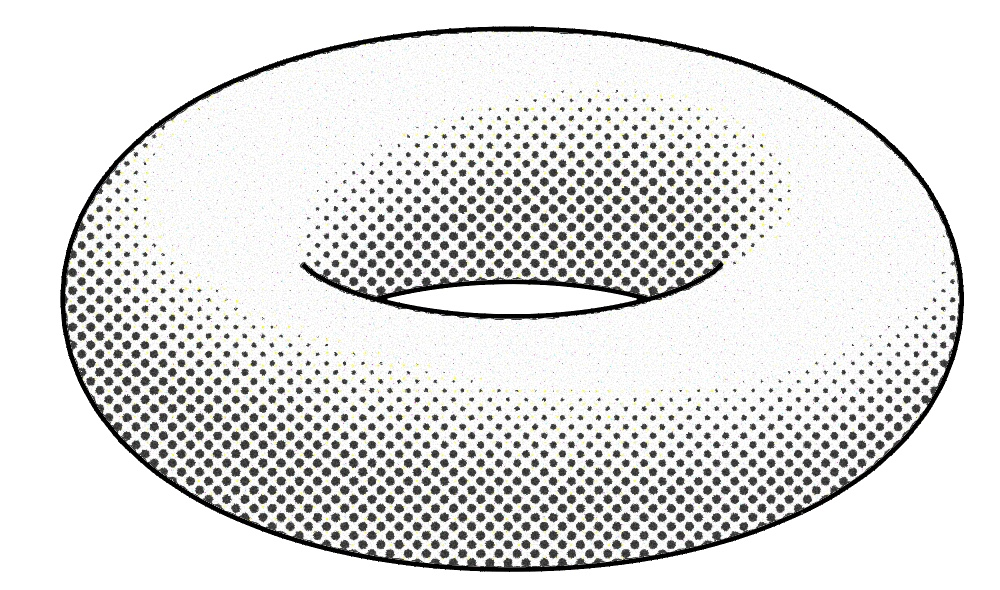
\includegraphics[scale=0.3]{graphics/diagrams/torus_non_vanishing_vector_field/result.jpg}
% 	\vspace{1em}
% 	\caption{A torus.}
% \end{figure}
%
% By relaxing our assumptions about the shape of space, geometry begins to quickly fill up with many such counter-intuitive non-Euclidean spaces and they find applications in unexpected places. Take for instance 
%
% \hspace{1em}
% % Many such axiomatic foundations exist, and lead 
%
% Let's start with the simple case of Euclidean space (think of a plane for instance) by describing some of its essential aspects. First and foremost Euclidean space is comprised of infinitely many points which \emph{extend continuously}, which informally means that Euclidean space is equipped with a qualitative concept of ``closeness''. Among other things, this 
%
% Euclidean space also comes with the stronger, quantitative notion of closeness -- this is known as \defn{distance}. A distance metric assigns to each pair of points a non-negative real number.

% \pagebreak

% \todo{The geometries they worked in were mostly flat, i.e. Euclidean and they relied on entirely (analytical?) methods to derive spatial relationships}
%
% \todo{Take a step back and see what data we have.}
%
% Classical geometry works in affine space, so we have: continuity of space, distance,  translation and homotethy. Translation gives us a global parallelism.
%
% Introduction of curvature
%
% Intrinstic  geometry via Theorema Egregium
%
% Symplectic manifolds, spin manifolds -> corresponding to physics
%
% Ehrlangen program

% At the scales they worked at, reality was best modelled by a plane or a (flat) three dimensional space.

% Homotopy classes of spaces
%
% PL manifolds
%
% During my last summer before graduating college, I went with some friends on a mountaineering trip up Banner peak, a picturesque mountain in the eastern Sierra Nevada range of California. 
% %
% % As we descended the glacier towards our base camp, ice axes in hand, I 
% So how \emph{do} we study objects which we can't touch, see, or possibly hope to visualize in their full complexity?
%
% There are two levels to understanding.
% \begin{enumerate}
% 	\item First, we
% \end{enumerate}
%
% Understanding an object by how it behaves with respect to other objects.
% \todo{spectral lines of atoms}
%
% One of the earliest methods to ``fingerprint'' topological objects was discovered by Euler.

% \cite{hatcher2002}
